\documentclass{llncs}
%\documentclass[a4paper]{article}

\usepackage{fullpage}
\usepackage{setspace}
\usepackage{url}
\usepackage{algorithmic}
\usepackage{algorithm}
\usepackage{amsmath}
\usepackage{latexsym}

\usepackage{graphicx}
\usepackage{subfig}

\onehalfspacing

%\newtheorem{definition}{Definition}
%\newtheorem{theorem}{Theorem}
%\newtheorem{example}{Example}
\newtheorem{query}{Query}

%\newcommand{\nop}[1]{}

\title{Mapping Microblogging Posts to Encyclopedia Articles}
\author{Uta L\"{o}sch \and David M\"{u}ller \and Andreas Harth}
\institute{
	Karlsruhe Institute of Technology (KIT), D-76131 Karlsruhe, Germany\\ 
	\email{uta.loesch@kit.edu},\\
	\email{david.mueller@student.kit.edu},\\
	\email{harth@kit.edu}
}
\begin{document}

\maketitle

\begin{abstract}
Search results on Twitter are hard to analyze and read. To facilitate understanding the meaning of a search term in the context of Twitter, we have developed a system which annotates search results with entities that best describe the search result, thus offering a means of quickly grasping the meaning of the search results and at the same time providing starting points for further exploration of the search results' context. In an evaluation we show that the entities used for annotation represent the tweet's content in a suitable manner and that the annotations remain stable over time, i.e. when executing the same search at different times, the same entities are returned.
\end{abstract}

\section{Introduction}

Twitter\footnote{\url{http://twitter.com}} is a micro-blogging service that has become very influential over the last years. The idea of micro-blogs is the same as that of blogs, except that the message length is restricted to 140 characters. Twitter has a total of about 190 million of users who produce 65 million tweets a day. Thus, Twitter represents a huge data source on the web.

Twitter offers the possibility to search for tweets containing a specific term or hash tags. This search returns a fixed number of most recent tweets containing the search term. However, it is hard to grasp the context of these tweets and to get further information on the topic that was searched for. As ach single tweet is very short and contains little information, it is necessary to parse the whole set in order to get an overview of the context(s) in which the search term is used. To facilitate this putting into context of the search results, we propose to annotate search results with a set of entities which reflect the content of the result feeds. These entities will not only help to understand the search terms, but also serve as a starting point when searching for further information related to the search result. This also helps to determine what the meaning of cryptic hash tags such as $\#s21$ or $\#ka$ mean. 

In this paper, we present a system which automatically annotates a Twitter search result with Wikipedia entities. While it would be more interesting to annotate each single tweet with relevant entities, tweets are too short to contain much relevant information which could be used as input for the annotation tool. Thus, we chose to generate annotations for the whole search result. 

The motivation for choosing Wikipedia entities was that it offers a wide coverage of topics. Furthermore, automatic tools for annotating text with Wikipedia entities are readily available (see \cite{key:wikifier}).

Annotations should be stable over time, unless the topics discussed in the tweets containing the search term change. In nan evaluation of our approach we have tried to analyse the stability of the result.

The rest of this paper is organized as follows: in Section~\ref{sect:method} we present our system, in Section~\ref{sect:eval} we present the results of our evaluation

\section{Method Overview}
\label{sect:method}

The implemented
system\footnote{\url{http://km.aifb.kit.edu/services/twittersearchwrap/}}
(further called Twitter Search Wrapper) is called with a query and returns a
rdf\footnote{\url{http://www.w3.org/RDF/}} document semantically describing the
most recent twitter posts (further called tweets) matching the given query. The returned rdf
document furthermore contains a mapping of the query to Encyclopedia articles
which based on the content published by users that most recently used the query
in their posts maps to articles best describing the content of tweets related to
the query. An overview of the System Architecture is given in Figure
\ref{fig:arch}. Taking a more detailed look, methods performed by the Twitter
Search Wrapper can be grouped into five sequential steps (see Figure
\ref{fig:arch}) .

 
\begin{figure}[htb]
  \centering
  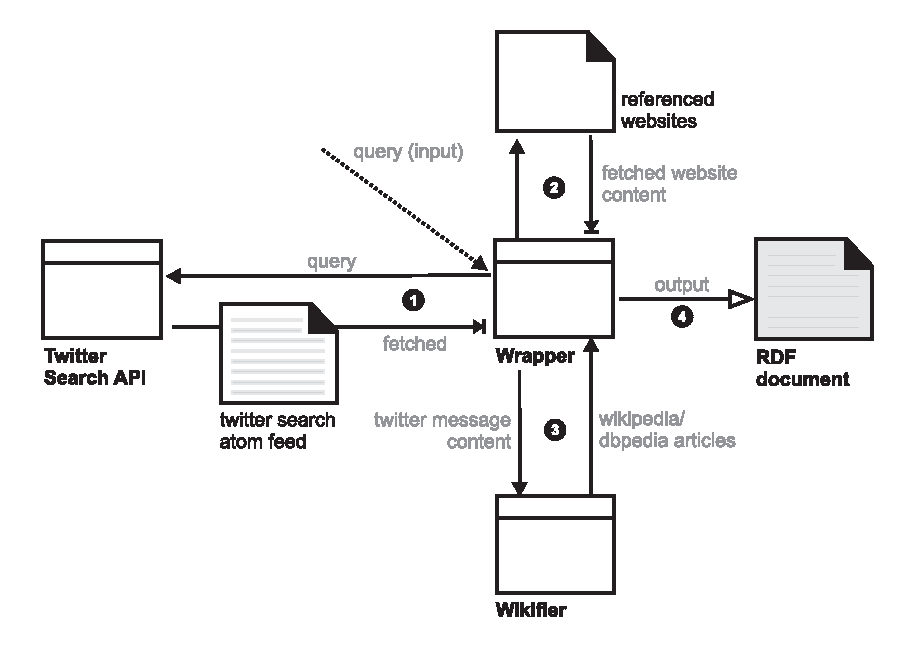
\includegraphics[width=.6\linewidth]{architecture}
  \caption{System Architecture}
  \label{fig:arch}
\end{figure}

In a first step the Twitter Search Wrapper fetches the atom feed
generated by the twitter search
api\footnote{\url{http://dev.twitter.com/doc/get/search}} for a given search
query. The generated feed contains information about the 100 most recently published publicly visible tweets and
their authors which match the search query. The tweets itself are described by
their content, publishing date, authors and optionally a geographic location. 

In a second (optional) step hyperlinks posted in tweets of the fetched
feed are followed, content of the referenced website's body is fetched and
processed to the Wrapper. This option is triggered calling the Twitter Search
Wrapper with attribute extern=true.

The Wrapper now calls the Wikifier \cite{key:wikifier} service. Content of the
tweets that matched the search query and optional content of their referenced websites is merged
to a single input string which is used as input for the Wikifier. The service
returns a list of matching articles of the English
Wikipedia. Optionally the wrapper can be initially called with lang=de to
trigger mapping to the German Wikipedia.

The list of matching Wikipedia articles is returned to the Wrapper. The Wrapper
generates a rdf document using popular ontologies (foaf, dublincore, geo) to
describe the data related to the returned tweets and their content including 'rdfs:seeAlso' links to
DBPedia\footnote{\url{http://dbpedia.org/About}} URIs (converted output of the
Wikifier) describing the documents content.

\section{Experiments and Evaluation}
\label{sect:eval}

Trending topics are listed in Table \ref{tbl:terms}.

\begin{table}[ht*]
\centering
\begin{tabular}{ c }
Search term                    \\
\hline
\#s21 \\
Karlsruhe\\
\end{tabular}
\caption{Search terms}\label{tbl:terms}
\end{table}

\begin{definition}[Stability]

\end{definition}

\section{Related Work}

Bringing Semantic Web technologies and Semantic Web technologies together, has been proposed before.

Passant et al. \cite{key:smob} have proposed a data model for making twitter
data available on the Semantic Web. They propose a data model which allows for the association of URIs with users, microblogs and microposts. To this end, SIOC and FOAF vocabularies are used and extended. Specifically, the new concepts \emph{Microblog} and {MicroBlogPost} are introduced. Additionally, they propose the use of so-called semantic hash tags. The idea is to use URIs as hash tags (e.g. \emph{\#geo:Paris\_France}). It becomes thus possible to link microposts to entities in the Linked Open Data cloud.
\section{Conclusion}





\bibliographystyle{abbrv}
\bibliography{bib}

\end{document}
